\documentclass[tikz,border=2pt]{standalone}
\usepackage[T1]{fontenc}
\usepackage{lmodern}
\usepackage{amsmath,amssymb}
\usetikzlibrary{arrows.meta,decorations.pathmorphing,decorations.pathreplacing,calc}
\definecolor{cblue}{HTML}{2b6cb0}
\definecolor{cdeep}{HTML}{1d4ed8}
\definecolor{cgold}{HTML}{b7791f}
\definecolor{cred}{HTML}{c0392b}
\definecolor{cgreen}{HTML}{1f8a5f}
\definecolor{tblue}{HTML}{e6eef8}
\definecolor{tgold}{HTML}{f8efdc}
\definecolor{tgray}{HTML}{efefef}
\definecolor{tgreen}{HTML}{e3f3eb}
\definecolor{cgray}{HTML}{8a8a8a}
\begin{document}
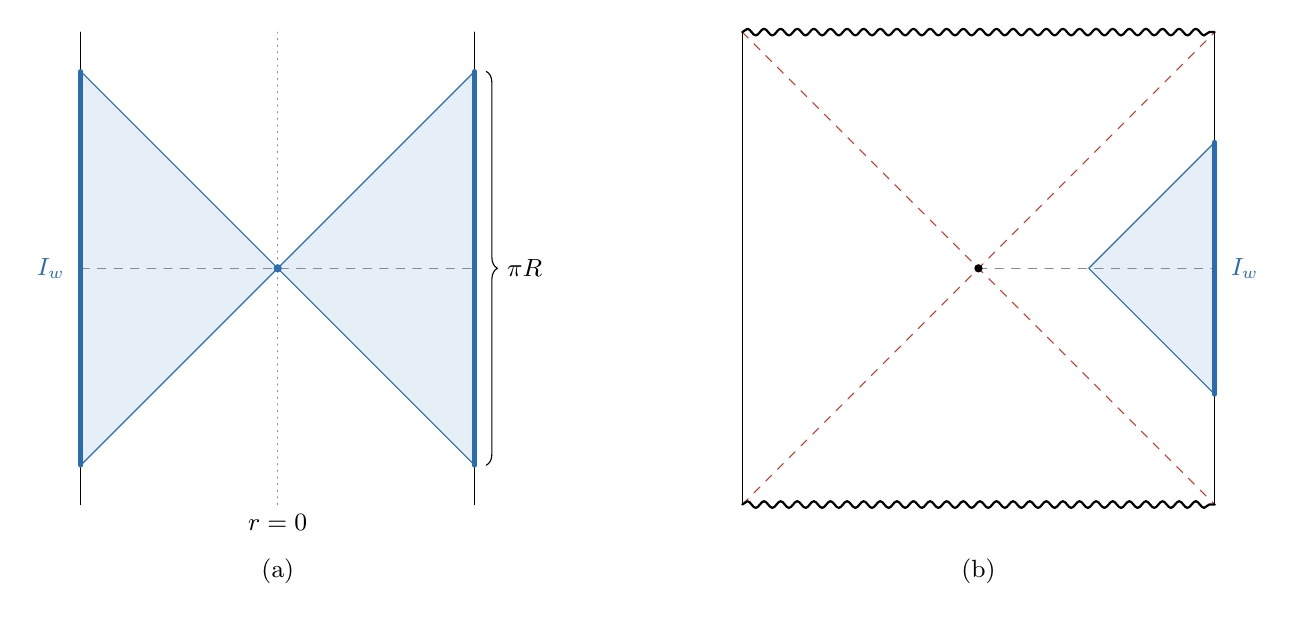
\begin{tikzpicture}[font=\small, line cap=round, line join=round]
  % ---------- (a) empty AdS (conformal strip, width pi R) ----------
  \def\a{2.5}
  \fill[tblue] (\a,\a) -- (0,0) -- (\a,-\a) -- cycle;
  \fill[tblue] (-\a,\a) -- (0,0) -- (-\a,-\a) -- cycle;
  \draw[cgray, dotted, thin] (0,-3) -- (0,3);
  \draw[cgray, dashed, thin] (-\a,0) -- (\a,0);
  \draw[cblue, thin] (\a,\a) -- (0,0) -- (\a,-\a);
  \draw[cblue, thin] (-\a,\a) -- (0,0) -- (-\a,-\a);
  \draw[thin] (-\a,-3) -- (-\a,3);
  \draw[thin] (\a,-3) -- (\a,3);
  \draw[cblue, line width=1.8pt] (\a,-\a) -- (\a,\a);
  \draw[cblue, line width=1.8pt] (-\a,-\a) -- (-\a,\a);
  \fill[cblue] (0,0) circle (1.5pt);
  \node[cblue, left] at (-\a-0.08,0) {$I_w$};
  \draw[decorate, decoration={brace, amplitude=4pt}, thin]
    (\a+0.15,\a) -- (\a+0.15,-\a) node[midway, right=4pt] {$\pi R$};
  \node[below] at (0,-3) {$r=0$};
  \node at (0,-3.85) {(a)};

  % ---------- (b) eternal black hole ----------
  \begin{scope}[shift={(8.9,0)}]
    \def\b{3}
    \def\w{1.6}
    \pgfmathsetmacro{\m}{\b-\w}
    \fill[tblue] (\b,\w) -- (\m,0) -- (\b,-\w) -- cycle;
    \draw[cgray, dashed, thin] (0,0) -- (\b,0);
    \draw[cblue, thin] (\b,\w) -- (\m,0) -- (\b,-\w);
    \draw[cred, dashed, thin] (-\b,-\b) -- (\b,\b);
    \draw[cred, dashed, thin] (-\b,\b) -- (\b,-\b);
    \draw[decorate, decoration={snake, segment length=6pt, amplitude=1.2pt}, thick]
      (-\b,\b) -- (\b,\b);
    \draw[decorate, decoration={snake, segment length=6pt, amplitude=1.2pt}, thick]
      (-\b,-\b) -- (\b,-\b);
    \draw[thin] (-\b,-\b) -- (-\b,\b);
    \draw[thin] (\b,-\b) -- (\b,\b);
    \draw[cblue, line width=1.8pt] (\b,-\w) -- (\b,\w);
    \fill (0,0) circle (1.5pt);
    \node[cblue, right] at (\b+0.08,0) {$I_w$};
    \node at (0,-3.85) {(b)};
  \end{scope}
\end{tikzpicture}
\end{document}
